\documentclass[11pt,a4paper]{report}
\usepackage[portuguese]{babel}
\usepackage{indentfirst}
\usepackage{mathptmx}
\usepackage[pt]{datetime2}
%\usepackage[utf8]{inputenc}
\usepackage{csquotes}
\usepackage{slantsc}
\usepackage[version=4]{mhchem}
%%%%%---------------------ESPAÇAMENTO E AVANÇO DE PARÁGRAFOS-------------------%%%%%%%%%
\usepackage{setspace}
\usepackage{emptypage}
\onehalfspacing
\setlength{\parindent}{1.25cm}
\setlength{\parskip}{6pt}
\newcommand{\newpara}
        {
        \vskip 6pt
        }
        
%%%%%--------------------------------------------------------------------------%%%%%%%%%
% Para gerar referências bibliográficas
\usepackage[style=apa]{biblatex}
\addbibresource{references.bib}

\usepackage{amsmath} % Para fórmulas matemáticas
\usepackage{hyperref, bookmark} % Para gerar os Índices
\hypersetup{pdfborder=0 0 0}
\usepackage{booktabs}


%%%%%-----------------------Referir-Figuras/Tabelas...---------------------------%%%%%%%%%
\usepackage[capitalize, brazilian]{cleveref}
% "cleveref" Portuguese names.
\Crefname{equation}{Equação}{Equações}
\Crefname{table}{Tabela}{Tabelas}
\Crefname{figure}{Figura}{Figuras}
\crefname{chapter}{capítulo}{capítulos}
\Crefname{chapter}{Capítulo}{Capítulos}
\crefname{section}{secção}{secções}
\Crefname{section}{Secção}{Secções}
\crefname{appendix}{anexo}{anexos}
\Crefname{appendix}{Anexo}{Anexos}
%%%%%--------------------------------------------------------------------------%%%%%%%%%

%%%%%--------------------------------MARGENS-----------------------------------%%%%%%%%%
\RequirePackage[outer=25mm,inner=35mm,vmargin=20mm,includehead,includefoot,headheight=15pt]{geometry}
\setlength{\headheight}{14pt} 

%%%%%---------------------------PERSONALIZAR TABELAS---------------------------%%%%%%%%%
\usepackage{array, multirow,multicol,tabularx,hhline}
\usepackage[table]{xcolor}
\newcolumntype{S}{>{\columncolor{black!20}} c}
\newcolumntype{Y}{>{\columncolor{yellow!20}} c}
\renewcommand{\arrayrulewidth}{0.2mm}
\newcolumntype{R}{>{\columncolor{red!30}} c}

\usepackage{caption}
\captionsetup[table]{skip=3pt}
\DeclareCaptionFormat{custom}
{%
    \textbf{#1#2}\emph{\small #3}
}
\captionsetup{format=custom}

\newcommand{\source}[1]{\caption*{\textbf{\normalsize{\emph{Fonte:}}} {#1}} }

%%%%%--------------------------------------------------------------------------%%%%%%%%%
\usepackage{graphicx} % Para introduzir imagens no documento
\graphicspath{{imagens/}} % Definir a pasta das imagens

%%%%%---------------------------------ESTILO 2---------------------------------%%%%%%%%%
\usepackage{fancyhdr}
\renewcommand{\chaptermark}[1]{\markboth{#1}{}}
\fancypagestyle{plain}{%  first page of chapters
    \fancyhf{} % clear all header and footer fields
    \fancyfoot[C]{\thepage}
    \renewcommand{\headrulewidth}{0pt} % no rule
    \renewcommand{\footrulewidth}{0pt} % Adicionar Linha no rodapé (Predefinição 0pt)
}
%\renewcommand{\sectionmark}[1]{ \markright{#1}{} }
\fancypagestyle{fancy}{%  all pages
    \fancyhf{} % clear all header and footer fields
    \fancyhead[L]{\textit{\small Teoria do Tratamento de Sinal}}
    \fancyhead[R]{\textit{\small Sá Pereira, J.}}
    \fancyfoot[C]{\thepage}
       \renewcommand{\headrulewidth}{0.5pt}
\renewcommand{\footrulewidth}{0pt}
}
 \pagestyle{fancy} % apply the stye <<<<<<<<<<<<<

 \usepackage[explicit,compact]{titlesec}
\titleformat{\chapter}[block]
    {\bfseries\huge}{\filright\huge\thechapter.}{1ex}{\huge\filright #1}
    \titlespacing*{\chapter}{0pt}{-30pt}{30pt}
\titlelabel{\thetitle.\quad}
\usepackage{subcaption}
\usepackage{hhline}
%%%%%--------------------------------------------------------------------------%%%%%%%%%

\setcounter{MaxMatrixCols}{20}
\usepackage{adjustbox}
\usepackage{float}
\usepackage{enumitem}
  \newcommand{\graus}{$^{\circ}$C }

  \usepackage{fontspec}
  \setmainfont{Calibri}
  \usepackage{lipsum}

\usepackage[numbered, framed]{matlab-prettifier}
\renewcommand{\lstlistingname}{Código}
\renewcommand{\lstlistlistingname}{Código}

%%%%%--------------------------------------------------------------------------%%%%%%%%%
%%%%%----------------------------ÍNICIO DO DOCUMENTO---------------------------%%%%%%%%%
%%%%%--------------------------------------------------------------------------%%%%%%%%%
\pagenumbering{roman}
\begin{document}
    \begin{titlepage}

    \newcommand{\HRule}{\rule{\linewidth}{0.4mm}} % Defines a new command for the horizontal lines, change thickness here
    
    \center      

    %	HEADING SECTIONS

    \textbf{\textsc{\Large Faculdade de Engenharia da Universidade do Porto}\\[2.5cm]}
    
\includegraphics[scale=.5]{uporto-feup.pdf}\\[2cm] 
    \textsc{\Large \bfseries Teoria do Tratamento de Sinal}\\[0.5cm] % Major heading such as course name
    \textsc{\large \bfseries M.EMG}\\[1cm] % Minor heading such as course title
    
    %	TITLE SECTION
    
    \HRule \\[0.4cm]
    { \LARGE{\bfseries Trabalho Final - \underline{Versão Provisória}}}\\[0.4cm] % Título
    \HRule \\[2cm]

    %	AUTHOR SECTION

    \begin{minipage}{0.4\textwidth}
        \begin{flushleft} \large
        \emph{Estudantes:}\\
        João \textsc{Sá Pereira} % Your name
        \end{flushleft}
        \end{minipage}
        ~
        \begin{minipage}{0.4\textwidth}
        \begin{flushright} \large
        \emph{Docentes:} \\
        Prof. Jorge \textsc{Carvalho} \\
        Prof. Teresa \textsc{Lajinha} % Supervisor's Name
        \end{flushright}
        \end{minipage}\\[2.5cm]
    
    % If you don't want a supervisor, uncomment the two lines below and remove the section above
    % \Large \emph{Estudante:}\\
    % João \textsc{Sá Pereira}\\[3cm] % Your name
    
    %	DATE SECTION
    \vfill
    {\large \today}\\[1cm]

 

        

    \end{titlepage}
    \shipout\null
    \pagestyle{plain}
%%%%%---------------------------------PREÂMBULO--------------------------------%%%%%%%%%
    %\cleardoublepage
    %\include{./capitulos/resumo}
    \cleardoublepage
    \pdfbookmark[0]{Conteúdo}{contents}
    \tableofcontents
    \cleardoublepage
    \pdfbookmark[0]{Lista de Figuras}{figures}
    \listoffigures
    % \cleardoublepage
    % \pdfbookmark[0]{Lista de Tabelas}{tables}
    % \listoftables
    \cleardoublepage
    \lstlistoflistings
    \cleardoublepage
%%%%%--------------------------------------------------------------------------%%%%%%%%%

%%%%%-----------------------------CORPO DO DOCUMENTO---------------------------%%%%%%%%%
\pagenumbering{arabic}
\pagestyle{fancy}
\chapter{Fourier Theory Made Easy (?)}
\section{Uma onda sinusoidal}

Começaremos por reproduzir uma onda sinusoidal. A sua forma mais básica, como função do tempo, é dada pela seguinte expressão:
\begin{equation}
    y(t) = A\cdot \sin \left(2\pi f t + \phi\right)
\end{equation}
% Onde:
% \begin{itemize}
%     \item $A=$ a amplitude;
%     \item $f=$ a frequência;
%     \item $2\pi f t= \omega = $ a frequência angular;
%     \item $\phi =$ a fase. 
% \end{itemize}

Para o primeiro exemplo, iremos representar em MATLAB uma onda sinusoidal com amplitude 5 e frequência de 4~Hz. Para isso, é necessário definir o eixo do tempo. Neste caso, o eixo do tempo começa em zero e acaba em 1 (segundos), com incrementos de 0.01. O código que fornece a imagem é o seguinte:

\newpara

\begin{lstlisting}[style=Matlab-editor, basicstyle=\small, label={lst: onda sinusoidal}]
dt = 0.01;
t = 0:dt:1;
F = 4;
A = 5;
y = A * sin(2 * pi * F * t);
plot(t,y);
xlabel('Segundos');
\end{lstlisting}

\begin{figure}[!ht]
\centering
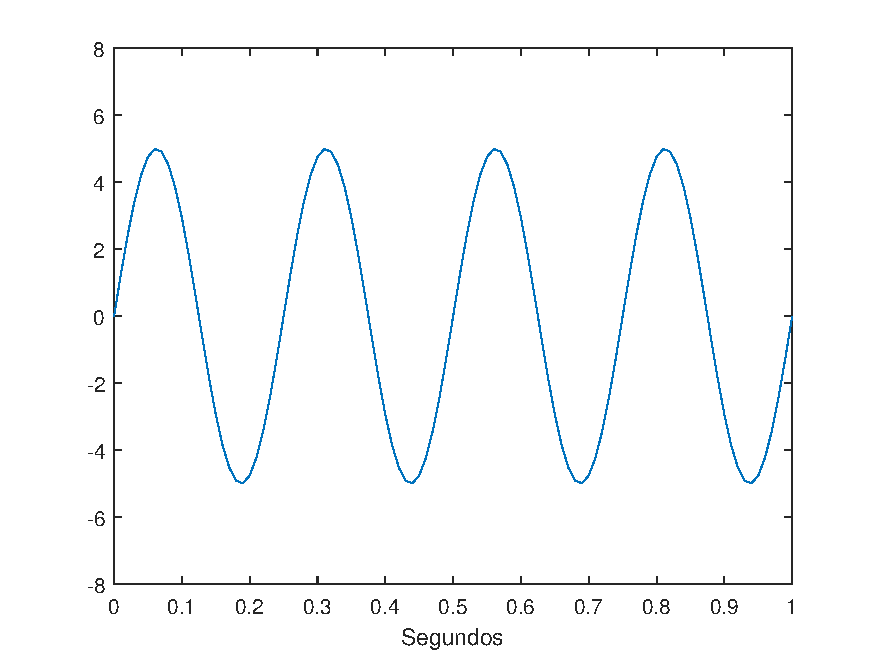
\includegraphics[width=0.75\textwidth]{onda sinusoidal.pdf}
\caption{Onda sinusoidal.}
\label{fig:onda sinusoidal}
\end{figure}

\newpage

Se definirmos a taxa de amostragem (\emph{sampling rate}) como sendo igual a 256 e a duração da amostragem (\emph{sampling duration}) como sendo igual a 1, podemos definir a variável dt como sendo o quociente entre a \emph{sampling duration} e o \emph{sampling rate}. E se representarmos a figura com pontos, podemos verificar que por cada segundo, temos 256 pontos.

\newpara

\begin{lstlisting}[style=Matlab-editor, basicstyle=\small, label={lst: sampling rate}]
sampling_rate = 256;
sampling_duration = 1; 
dt = sampling_duration/sampling_rate;
t = 0:dt:1;
F = 4;
A = 5;
y = A * sin(2 * pi * F * t);
plot(t, y, 'o', 'MarkerSize',4);
xlabel('Segundos')
\end{lstlisting}
    
\begin{figure}[!ht]
\centering
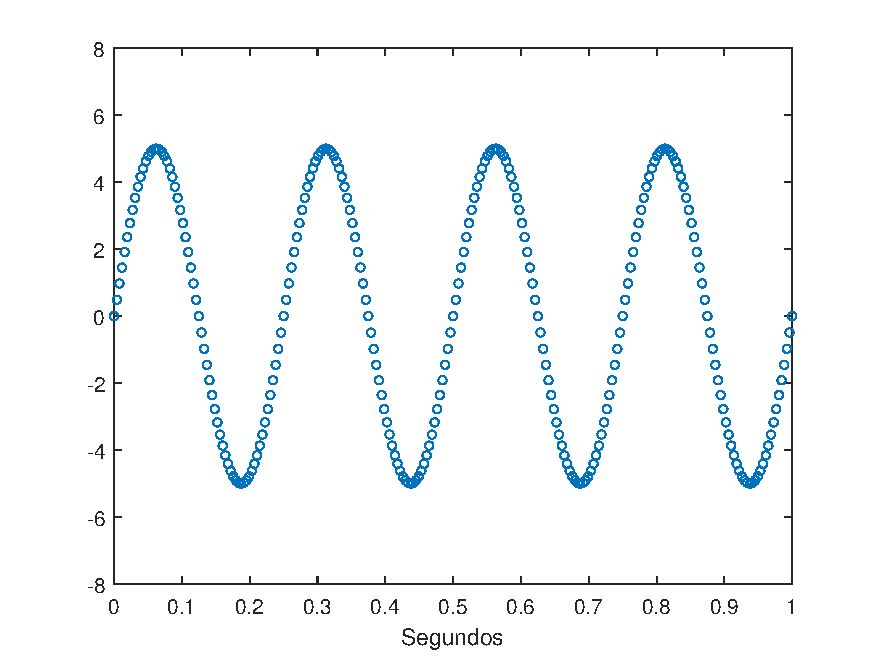
\includegraphics[width=0.75\textwidth]{samplingrate.pdf}
\caption{Taxa de amostragem.}
\label{fig:sampling rate}
\end{figure}

Agora uma função sinusoidal com frequência de 8~Hz e com uma determinada taxa de amostragem. Quando se altera o valor do passo de amostragem, para 8.5~Hz, obtêm-se um sinal com frequência de 0.5~Hz. Este exercicio, recriado em MATLAB no código da página seguinte, mostra a importância da escolha do passo de amostragem.

% Se sobrepusermos dois gráficos, um com uma taxa de amostragem muito pequena, por exemplo 8.5, e outro com uma taxa de amostragem maior, por exemplo 256, é possível verificar o efeito da taxa de amostragem. Para um eixo do tempo de dois segundos, verifica-se, na \autoref{fig:undersampled}, que no sinal subamostrado temos 18 pontos representados. 

\newpage

\lstinputlisting[style=Matlab-editor, basicstyle=\small, label={lst: undersampled}, firstline=2]{./codigo/undersampled.m}

\begin{figure}[!ht]
\centering
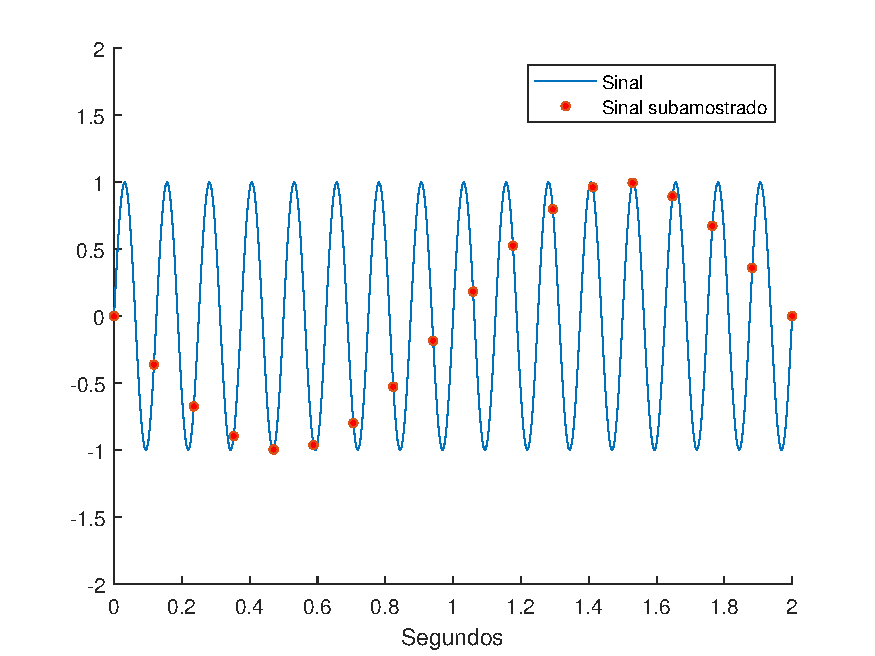
\includegraphics[width=0.75\textwidth]{undersampled.pdf}
\caption{Sinal subamostrado.}
\label{fig:undersampled}
\end{figure}

\newpage

\section{Transformadas de Fourier Famosas}

Uma transformada pega numa função (ou sinal) e transforma-a numa outra função (ou sinal).
A transformada discreta de Fourier é dada pela seguinte expressão:
\begin{equation}
    H(f)=\int_{-\infty}^{+\infty} h(t)\cdot e^{2\pi ift} \cdot dt 
\end{equation}

A transformada rápida de Fourier (do inglês: \emph{Fast Fourier Transform}, abreviado FFT), é um algoritmo que calcula a transformada discreta de Fourier. A análise de Fourier converte um sinal do domínio original (tempo) para uma representação no domínio das frequências e vice-versa.

\subsection{Função Seno \boldmath{$\rightarrow$} Função Delta} 

A transformada de Fourier de uma função sinusoidal é uma função delta de Dirac, pelo menos em parte. Quando aplicamos a transformada de Fourier no MATLAB (função \emph{fft}) a uma função sinusoidal, o resultado é uma combinação de deltas de Dirac localizados nas frequências da função sinusoidal. A transformada de Fourier da função é zero em todas as frequências exceto na frequência da função seno, onde há um Dirac localizado.

\newpara
\lstinputlisting[style=Matlab-editor, basicstyle=\small, label={lst: seno_delta}, firstline=2]{./codigo/seno_delta.m}

\newpage

É possível verificar pelos gráficos produzidos pelo código anterior, que o Dirac ocorre na frequência $7.98403\approx 8$, que é a frequência da função sinusoidal.

\begin{figure}[!ht]
    \centering
    \begin{minipage}[b]{0.49\textwidth}
        \centering
        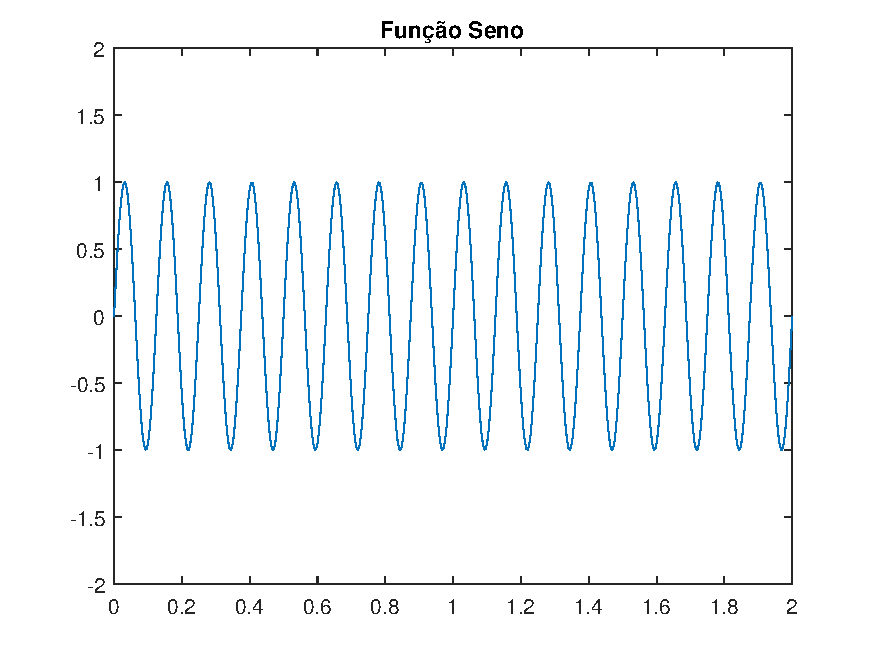
\includegraphics[width=\textwidth]{função seno.pdf}
        \caption{Função Seno.}
    \end{minipage}
    \hfill
    \begin{minipage}[b]{0.49\textwidth}
        \centering
        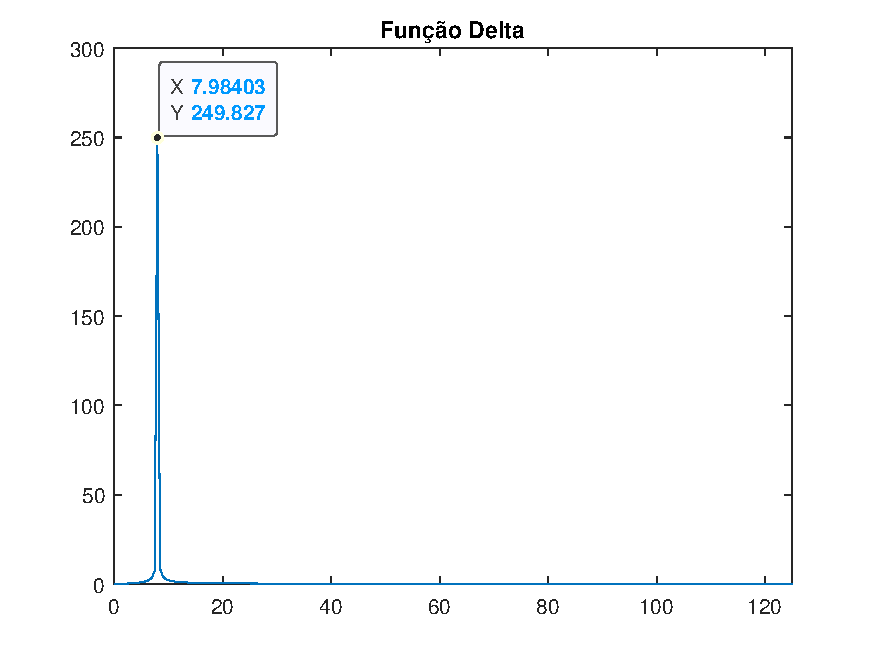
\includegraphics[width=\textwidth]{função delta.pdf}
        \caption{Função Delta.}
    \end{minipage}
\end{figure}

\subsection{Função Gaussiana}

A transformada de Fourier de uma função gaussiana é também uma função gaussiana mas com parâmetros diferentes.

\newpara
\lstinputlisting[style=Matlab-editor, basicstyle=\small, label={lst: gauss}, firstline=2]{./codigo/gauss.m}

Neste caso, a amplitude da transformada de Fourier é 5 e a média é 125. As figuras da página seguinte mostram a resposta do código apresentado.

\newpage

\begin{figure}[!ht]
    \centering
    \begin{minipage}[b]{0.49\textwidth}
        \centering
        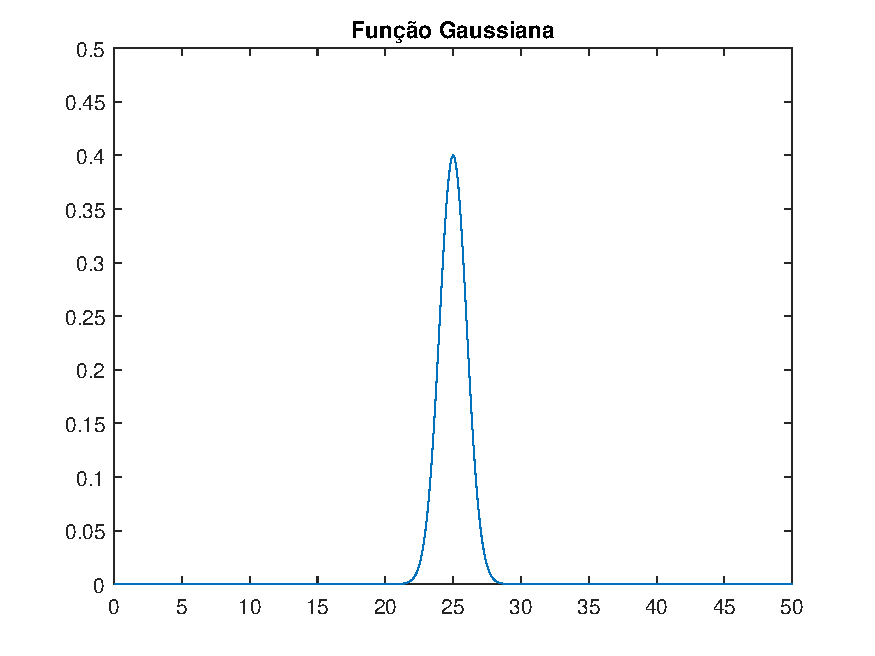
\includegraphics[width=\textwidth]{gauss.pdf}
        \caption{Função Gaussiana.}
    \end{minipage}
    \hfill
    \begin{minipage}[b]{0.49\textwidth}
        \centering
        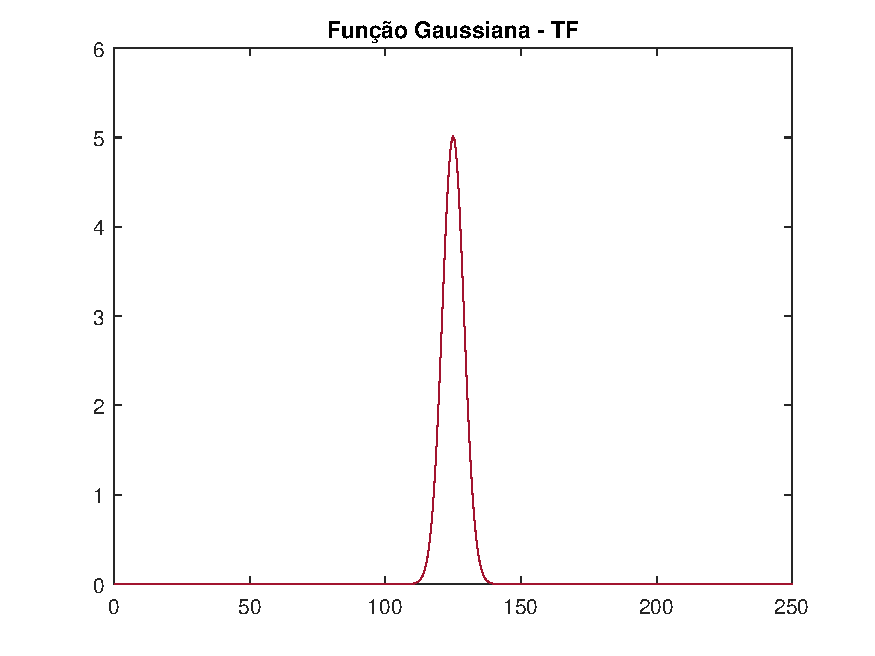
\includegraphics[width=\textwidth]{gaussTF.pdf}
        \caption{Função Gaussiana - TF.}
    \end{minipage}
\end{figure}

\subsection{Função Seno Cardinal \boldmath{$\rightarrow$} Pedestal}

Isto é apenas um teste meu amigo.

%\include{./capitulos/capitulo2}
%\include{./capitulos/capitulo3}
% \include{./capitulos/capitulo4}
%%%%%--------------------------------------------------------------------------%%%%%%%%%

%%%%%--------------------------BIBLIOGRAFIA E ANEXOS---------------------------%%%%%%%%%
% \nocite{*}
% \printbibliography % Gera as Referências Bibliográficas

%%%%%--------------------------------------------------------------------------%%%%%%%%%
%\appendix
%\input{anexos}

%%%%%--------------------------------------------------------------------------%%%%%%%%%
\end{document}
